% GNUPLOT: LaTeX picture with Postscript
\begingroup
  \makeatletter
  \providecommand\color[2][]{%
    \GenericError{(gnuplot) \space\space\space\@spaces}{%
      Package color not loaded in conjunction with
      terminal option `colourtext'%
    }{See the gnuplot documentation for explanation.%
    }{Either use `blacktext' in gnuplot or load the package
      color.sty in LaTeX.}%
    \renewcommand\color[2][]{}%
  }%
  \providecommand\includegraphics[2][]{%
    \GenericError{(gnuplot) \space\space\space\@spaces}{%
      Package graphicx or graphics not loaded%
    }{See the gnuplot documentation for explanation.%
    }{The gnuplot epslatex terminal needs graphicx.sty or graphics.sty.}%
    \renewcommand\includegraphics[2][]{}%
  }%
  \providecommand\rotatebox[2]{#2}%
  \@ifundefined{ifGPcolor}{%
    \newif\ifGPcolor{}
    \GPcolortrue{}
  }{}%
  \@ifundefined{ifGPblacktext}{%
    \newif\ifGPblacktext{}
    \GPblacktexttrue{}
  }{}%
  % define a \g@addto@macro without @ in the name:
  \let\gplgaddtomacro\g@addto@macro{}
  % define empty templates for all commands taking text:
  \gdef\gplbacktext{}%
  \gdef\gplfronttext{}%
  \makeatother
  \ifGPblacktext{}
    % no textcolor at all
    \def\colorrgb#1{}%
    \def\colorgray#1{}%
  \else
    % gray or color?
    \ifGPcolor{}
      \def\colorrgb#1{\color[rgb]{#1}}%
      \def\colorgray#1{\color[gray]{#1}}%
      \expandafter\def\csname LTw\endcsname{\color{white}}%
      \expandafter\def\csname LTb\endcsname{\color{black}}%
      \expandafter\def\csname LTa\endcsname{\color{black}}%
      \expandafter\def\csname LT0\endcsname{\color[rgb]{1,0,0}}%
      \expandafter\def\csname LT1\endcsname{\color[rgb]{0,1,0}}%
      \expandafter\def\csname LT2\endcsname{\color[rgb]{0,0,1}}%
      \expandafter\def\csname LT3\endcsname{\color[rgb]{1,0,1}}%
      \expandafter\def\csname LT4\endcsname{\color[rgb]{0,1,1}}%
      \expandafter\def\csname LT5\endcsname{\color[rgb]{1,1,0}}%
      \expandafter\def\csname LT6\endcsname{\color[rgb]{0,0,0}}%
      \expandafter\def\csname LT7\endcsname{\color[rgb]{1,0.3,0}}%
      \expandafter\def\csname LT8\endcsname{\color[rgb]{0.5,0.5,0.5}}%
    \else
      % gray
      \def\colorrgb#1{\color{black}}%
      \def\colorgray#1{\color[gray]{#1}}%
      \expandafter\def\csname LTw\endcsname{\color{white}}%
      \expandafter\def\csname LTb\endcsname{\color{black}}%
      \expandafter\def\csname LTa\endcsname{\color{black}}%
      \expandafter\def\csname LT0\endcsname{\color{black}}%
      \expandafter\def\csname LT1\endcsname{\color{black}}%
      \expandafter\def\csname LT2\endcsname{\color{black}}%
      \expandafter\def\csname LT3\endcsname{\color{black}}%
      \expandafter\def\csname LT4\endcsname{\color{black}}%
      \expandafter\def\csname LT5\endcsname{\color{black}}%
      \expandafter\def\csname LT6\endcsname{\color{black}}%
      \expandafter\def\csname LT7\endcsname{\color{black}}%
      \expandafter\def\csname LT8\endcsname{\color{black}}%
    \fi
  \fi
    \setlength{\unitlength}{0.0500bp}%
    \ifx\gptboxheight\undefined%
      \newlength{\gptboxheight}%
      \newlength{\gptboxwidth}%
      \newsavebox{\gptboxtext}%
    \fi%
    \setlength{\fboxrule}{0.5pt}%
    \setlength{\fboxsep}{1pt}%
\begin{picture}(5760.00,2880.00)%
    \gplgaddtomacro\gplbacktext{%
      \csname LTb\endcsname%
      \put(156,704){\makebox(0,0)[r]{\strut{}\(0.0x10^{0}\)}}%
      \put(156,972){\makebox(0,0)[r]{\strut{}\(1.0x10^{4}\)}}%
      \put(156,1241){\makebox(0,0)[r]{\strut{}\(2.0x10^{4}\)}}%
      \put(156,1509){\makebox(0,0)[r]{\strut{}\(3.0x10^{4}\)}}%
      \put(156,1777){\makebox(0,0)[r]{\strut{}\(4.0x10^{4}\)}}%
      \put(156,2045){\makebox(0,0)[r]{\strut{}\(5.0x10^{4}\)}}%
      \put(156,2314){\makebox(0,0)[r]{\strut{}\(6.0x10^{4}\)}}%
      \put(156,2582){\makebox(0,0)[r]{\strut{}\(7.0x10^{4}\)}}%
      \put(156,2850){\makebox(0,0)[r]{\strut{}\(8.0x10^{4}\)}}%
      \put(744,484){\makebox(0,0){\strut{}\(2.0\)}}%
      \put(1200,484){\makebox(0,0){\strut{}\(2.5\)}}%
      \put(1656,484){\makebox(0,0){\strut{}\(3.0\)}}%
      \put(2112,484){\makebox(0,0){\strut{}\(4.0\)}}%
      \put(2568,484){\makebox(0,0){\strut{}\(6.0\)}}%
      \put(3024,484){\makebox(0,0){\strut{}\(8.0\)}}%
      \put(3479,484){\makebox(0,0){\strut{}\(10.0\)}}%
      \put(3935,484){\makebox(0,0){\strut{}\(12.0\)}}%
      \put(4391,484){\makebox(0,0){\strut{}\(14.0\)}}%
      \put(4847,484){\makebox(0,0){\strut{}\(16.0\)}}%
      \put(5303,484){\makebox(0,0){\strut{}\(18.0\)}}%
    }%
    \gplgaddtomacro\gplfronttext{%
      \csname LTb\endcsname%
      \put(-746,1777){\rotatebox{-270}{\makebox(0,0){\strut{}Synapses}}}%
      \put(3023,154){\makebox(0,0){\strut{}Time (\(x 1000s\))}}%
      \csname LTb\endcsname%
      \put(2564,2707){\makebox(0,0)[r]{\strut{}Other}}%
      \csname LTb\endcsname%
      \put(2564,2487){\makebox(0,0)[r]{\strut{}Peri LPZ}}%
      \csname LTb\endcsname%
      \put(3947,2707){\makebox(0,0)[r]{\strut{}LPZ B}}%
      \csname LTb\endcsname%
      \put(3947,2487){\makebox(0,0)[r]{\strut{}LPZ C}}%
    }%
    \gplbacktext
    \put(0,0){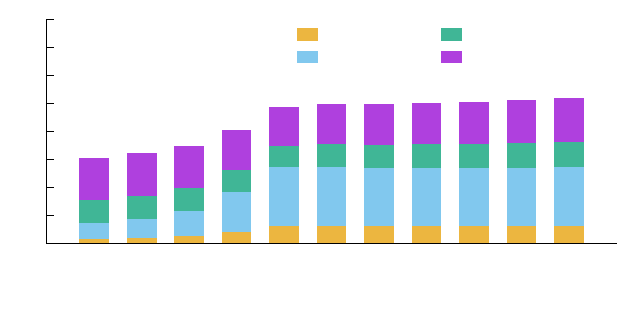
\includegraphics{99_images/201908061027-75-connection-rowstacked-histograms-E-to-lpz_c_E}}%
    \gplfronttext
  \end{picture}%
\endgroup
